% KTH master's thesis presentation, converted from V2.pptx.
% Figures are the thesis assets in ../figures (TikZ sources and experiment plots).
%
%   cd presentation
%   pdflatex -interaction=nonstopmode -output-directory=build kth-presentation.tex
%   pdflatex -interaction=nonstopmode -output-directory=build kth-presentation.tex
\documentclass[aspectratio=169,10pt]{beamer}

\usepackage{amsmath,amssymb,bm,booktabs,mathtools}
\usepackage{tikz}
\usetikzlibrary{positioning,arrows.meta,calc,fit,shapes.geometric,patterns,decorations.pathreplacing}

\graphicspath{{../figures/}}

% Macros the shared TikZ figures expect. Acronyms are expanded in place
% so the figures compile without the thesis glossary.
\newcommand{\R}{\mathbb{R}}
\newcommand{\vect}[1]{\bm{#1}}
\newcommand{\mat}[1]{\bm{#1}}
\newcommand{\Loss}{\mathcal{L}}
\makeatletter
\newcommand{\gls}[1]{\csname briefgls@#1\endcsname}
\newcommand{\Gls}[1]{\csname briefgls@#1\endcsname}
\newcommand{\glspl}[1]{\csname briefglspl@#1\endcsname}
\newcommand{\briefgls@pdw}{PDW}
\newcommand{\briefglspl@pdw}{PDWs}
\newcommand{\briefgls@dbscan}{DBSCAN}
\newcommand{\briefgls@toa}{TOA}
\makeatother

\definecolor{kthblue}{RGB}{25,84,166}
\definecolor{kthlight}{RGB}{232,240,250}
\definecolor{saaborange}{RGB}{196,90,22}

\usetheme{default}
\usecolortheme{default}
\setbeamercolor{structure}{fg=kthblue}
\setbeamercolor{frametitle}{bg=kthblue,fg=white}
\setbeamercolor{title}{fg=kthblue}
\setbeamercolor{block title}{bg=kthblue,fg=white}
\setbeamercolor{block body}{bg=kthlight,fg=black}
\setbeamercolor{block title alerted}{bg=saaborange,fg=white}
\setbeamercolor{block body alerted}{bg=saaborange!8,fg=black}
\setbeamerfont{frametitle}{series=\bfseries,size=\large}
\setbeamerfont{title}{series=\bfseries,size=\Large}
\setbeamertemplate{navigation symbols}{}
\setbeamertemplate{itemize item}{\textcolor{kthblue}{\textbullet}}
\setbeamertemplate{itemize subitem}{\textcolor{kthblue}{--}}
\setbeamersize{text margin left=5.5mm,text margin right=5.5mm}

\setbeamertemplate{frametitle}{%
  \expandafter\ifblank\expandafter{\insertframetitle}{}{%
    \nointerlineskip
    \begin{beamercolorbox}[wd=\paperwidth,ht=3.6ex,dp=1.5ex,leftskip=5.5mm,rightskip=5.5mm]{frametitle}%
      \usebeamerfont{frametitle}\insertframetitle
    \end{beamercolorbox}%
  }%
}

\setbeamertemplate{footline}{%
  \leavevmode
  \hbox{%
    \begin{beamercolorbox}[wd=\paperwidth,ht=2.5ex,dp=1.1ex,leftskip=5.5mm,rightskip=5.5mm]{frametitle}%
      \usebeamerfont{footline}\color{white!85}\scriptsize
      Master's thesis presentation \quad KTH EECS \quad Saab \quad Markus Johnson Swegmark
      \hfill
      \insertframenumber\,/\,\inserttotalframenumber
    \end{beamercolorbox}%
  }%
}

\newcommand{\thesisfig}[3]{%
  \resizebox{#1}{#2}{\input{#3}}%
}
\DeclareMathOperator{\softmax}{softmax}

% Pairwise-bias schematic used on the physical-bias frame.
% Cell color tracks absolute pairwise difference.
\newcommand{\deltagrid}[1]{%
  \begin{tikzpicture}[x=0.42cm,y=0.42cm,baseline=-0.5ex]
    \foreach \i in {0,...,4} {%
      \foreach \j in {0,...,4} {%
        \pgfmathtruncatemacro{\tone}{12+20*abs(\i-\j)}%
        \fill[#1!\tone] (\j,-\i) rectangle ++(0.92,-0.92);%
      }%
    }%
  \end{tikzpicture}%
}
\newcommand{\groupgrid}[1]{%
  \begin{tikzpicture}[x=0.42cm,y=0.42cm,baseline=-0.5ex]
    \foreach \i in {0,...,4} {%
      \foreach \j in {0,...,4} {%
        \pgfmathtruncatemacro{\tone}{int(abs(\i-\j)<2 ? 18 : 78)}%
        \fill[#1!\tone] (\j,-\i) rectangle ++(0.92,-0.92);%
      }%
    }%
  \end{tikzpicture}%
}

\title{Joint Radar Emitter and Mode Clustering Using Transformer Encoder Architecture}
\author{Markus Johnson Swegmark}
\institute{Saab \quad KTH Royal Institute of Technology}
\date{Master's thesis presentation}

\begin{document}

% ---------------------------------------------------------------------
\begin{frame}
  \vfill
  \begin{columns}[c]
    \begin{column}{0.72\textwidth}
      {\usebeamercolor[fg]{title}\LARGE\bfseries
        Joint Radar Emitter and Mode\\[0.25em]
        Clustering Using Transformer\\[0.25em]
        Encoder Architecture\par}
      \vspace{6mm}
      {\large Markus Johnson Swegmark\par}
      \vspace{1.5mm}
      {\normalsize Degree project in Machine Learning, 30 credits\\[0.1em]
        School of Electrical Engineering and Computer Science\\[0.1em]
        KTH Royal Institute of Technology\par}
      \vspace{2.5mm}
      {\normalsize
        Supervisors: Alexander Karlsson, Elin Ohlman (Saab)\\[0.12em]
        Saikat Chatterjee (KTH)\\[0.12em]
        Examiner: Magnus Jansson \quad Host: Saab AB\par}
    \end{column}
    \begin{column}{0.24\textwidth}
      \centering
      
\includegraphics[width=\linewidth]{kth/KTH_logo_RGB_bla.png}
    \end{column}
  \end{columns}
  \vfill
  \note{Degree-project presentation. Data and the two attention variants come first.}
\end{frame}

% ---------------------------------------------------------------------
\begin{frame}{The situation}
  \begin{columns}[c]
    \begin{column}{0.60\textwidth}
      \centering
      \thesisfig{\linewidth}{!}{../figures/background/esm_scene.tex}
    \end{column}
    \begin{column}{0.37\textwidth}
      \begin{itemize}
        \item The own platform listens and does not transmit.
        \item Several emitters radiate at once.
        \item One mixed stream of pulses arrives.
      \end{itemize}
    \end{column}
  \end{columns}
  \note{If you turn on your own radar, you light up the scene, and anyone listening knows you are there. The alternative is to stay quiet and record what others transmit. Several radars transmit at once, so the recording is one mixed list of pulses. The task is to say which pulses come from the same radar, and which operating mode that radar is using.}
\end{frame}

% ---------------------------------------------------------------------
\begin{frame}{Terminology}
  \textbf{Electronic Support Measures (ESM)}\\[0.2em]
  The listener. It detects, intercepts, and analyzes electromagnetic signals without transmitting.

  \vspace{0.7em}
  \textbf{Pulse Descriptor Word (PDW)}\\[0.2em]
  One measured pulse, stored as a discrete record of its parameters.

  \vspace{0.8em}
  \begin{columns}[T]
    \begin{column}{0.48\textwidth}
      \begin{itemize}
        \item Time of arrival (TOA)
        \item Carrier frequency
        \item Pulse width (PW)
      \end{itemize}
    \end{column}
    \begin{column}{0.48\textwidth}
      \begin{itemize}
        \item Amplitude
        \item Angle of arrival (AOA)\\
              {\footnotesize Direction the pulse came from.}
      \end{itemize}
    \end{column}
  \end{columns}
\end{frame}

% ---------------------------------------------------------------------
\begin{frame}{Problem}
  A typical ESM processing chain:

  \vspace{0.5em}
  \centering
  \thesisfig{0.92\textwidth}{!}{../figures/background/classical_pipeline.tex}

  \vspace{0.7em}
  \raggedright
  \begin{itemize}
    \item Mode classification runs on deinterleaved streams, so it sees less of the mixture. Pulses dropped by a poor deinterleaving never reach it.
    \item A classifier does not handle new emitters naturally. Clustering is the broader alternative.
  \end{itemize}

  \vspace{0.4em}
  \begin{block}{Hypothesis}
    Joint deinterleaving and mode clustering can do better: one model for both.
  \end{block}
\end{frame}

% ---------------------------------------------------------------------
\begin{frame}{Operating modes}
  \centering
  \thesisfig{0.96\textwidth}{!}{../figures/background/mode_patterns.tex}
  \note{A mode is the radar's transmit schedule, not a second radar. Search is slow and steady. Track is the same rhythm, faster. Stagger alternates the gap. Scan sends a burst and then goes quiet. One emitter can switch among these. The next slide is what arrives when several emitters do this at once.}
\end{frame}

% ---------------------------------------------------------------------
\begin{frame}{One mixed stream, two partitions}
  \centering
  \thesisfig{0.86\textwidth}{!}{../figures/method/partitions.tex}

  \vspace{0.15em}
  \begin{columns}[T]
    \begin{column}{0.48\textwidth}
      \textbf{Emitter \textperiodcentered\ deinterleaving}
      \begin{itemize}
        \item Physical source
        \item Cluster within the recording
        \item What classical deinterleaving recovers
      \end{itemize}
    \end{column}
    \begin{column}{0.48\textwidth}
      \textbf{Mode \textperiodcentered\ operating schedule}
      \begin{itemize}
        \item Operating mode
        \item One mode can sit on several emitters; one emitter can switch modes
        \item Inference clusters. The catalogue is used in training, not at inference
      \end{itemize}
    \end{column}
  \end{columns}
  \note{The classical chain deinterleaves first. Both partitions are read off the mixed list.}
\end{frame}

% ---------------------------------------------------------------------
\begin{frame}{Research questions}
  \textbf{RQ1.} Given a bounded window of PDWs, can a transformer encoder deinterleave pulses and recover operating modes by clustering?

  \vspace{0.7em}
  \textbf{RQ2.} Does a joint objective that couples deinterleaving with mode clustering outperform a comparable transformer trained for deinterleaving alone?

  \vspace{0.7em}
  \textbf{RQ3.} Do a pairwise physical attention bias and rotary positional encoding on pulse coordinates improve clustering relative to standard multi-head attention?
\end{frame}

% ---------------------------------------------------------------------
\begin{frame}{Data}
  \begin{itemize}
    \item Generated with Saab's scenario simulator.
    \item 1950 scenarios: 1461 train, 245 validation, and 244 test. Catalogue of 19 modes.
    \item Scenarios are cut into windows of length \(L = 2000\) so they fit the transformer.
  \end{itemize}

  \vspace{0.4em}
  \centering
  {\small
  \begin{tabular}{@{}lccccc@{}}
    \toprule
    Split & Scenarios & Pulses & Windows & Emitters & Modes \\
    \midrule
    Train      & 1461 & \(13.8 \times 10^{6}\) & 56\,029 & \(3.15 \pm 1.14\) & \(6.16 \pm 2.95\) \\
    Validation & 245  & \(2.25 \times 10^{6}\) & 1\,107  & \(3.16 \pm 1.21\) & \(6.18 \pm 2.95\) \\
    Test       & 244  & \(2.36 \times 10^{6}\) & 1\,169  & \(3.17 \pm 1.20\) & \(6.18 \pm 3.02\) \\
    \bottomrule
  \end{tabular}}

  \vspace{0.45em}
  {\footnotesize Emitter and mode columns are mean \(\pm\) std distinct labels per window.
  Training windows overlap; validation and test windows do not.}
\end{frame}

% ---------------------------------------------------------------------
\begin{frame}{Examples of scenarios}
  \begin{columns}[T,onlytextwidth]
    \begin{column}{0.33\textwidth}
      \centering
      {\small\bfseries Crowded}\\[0.25em]
      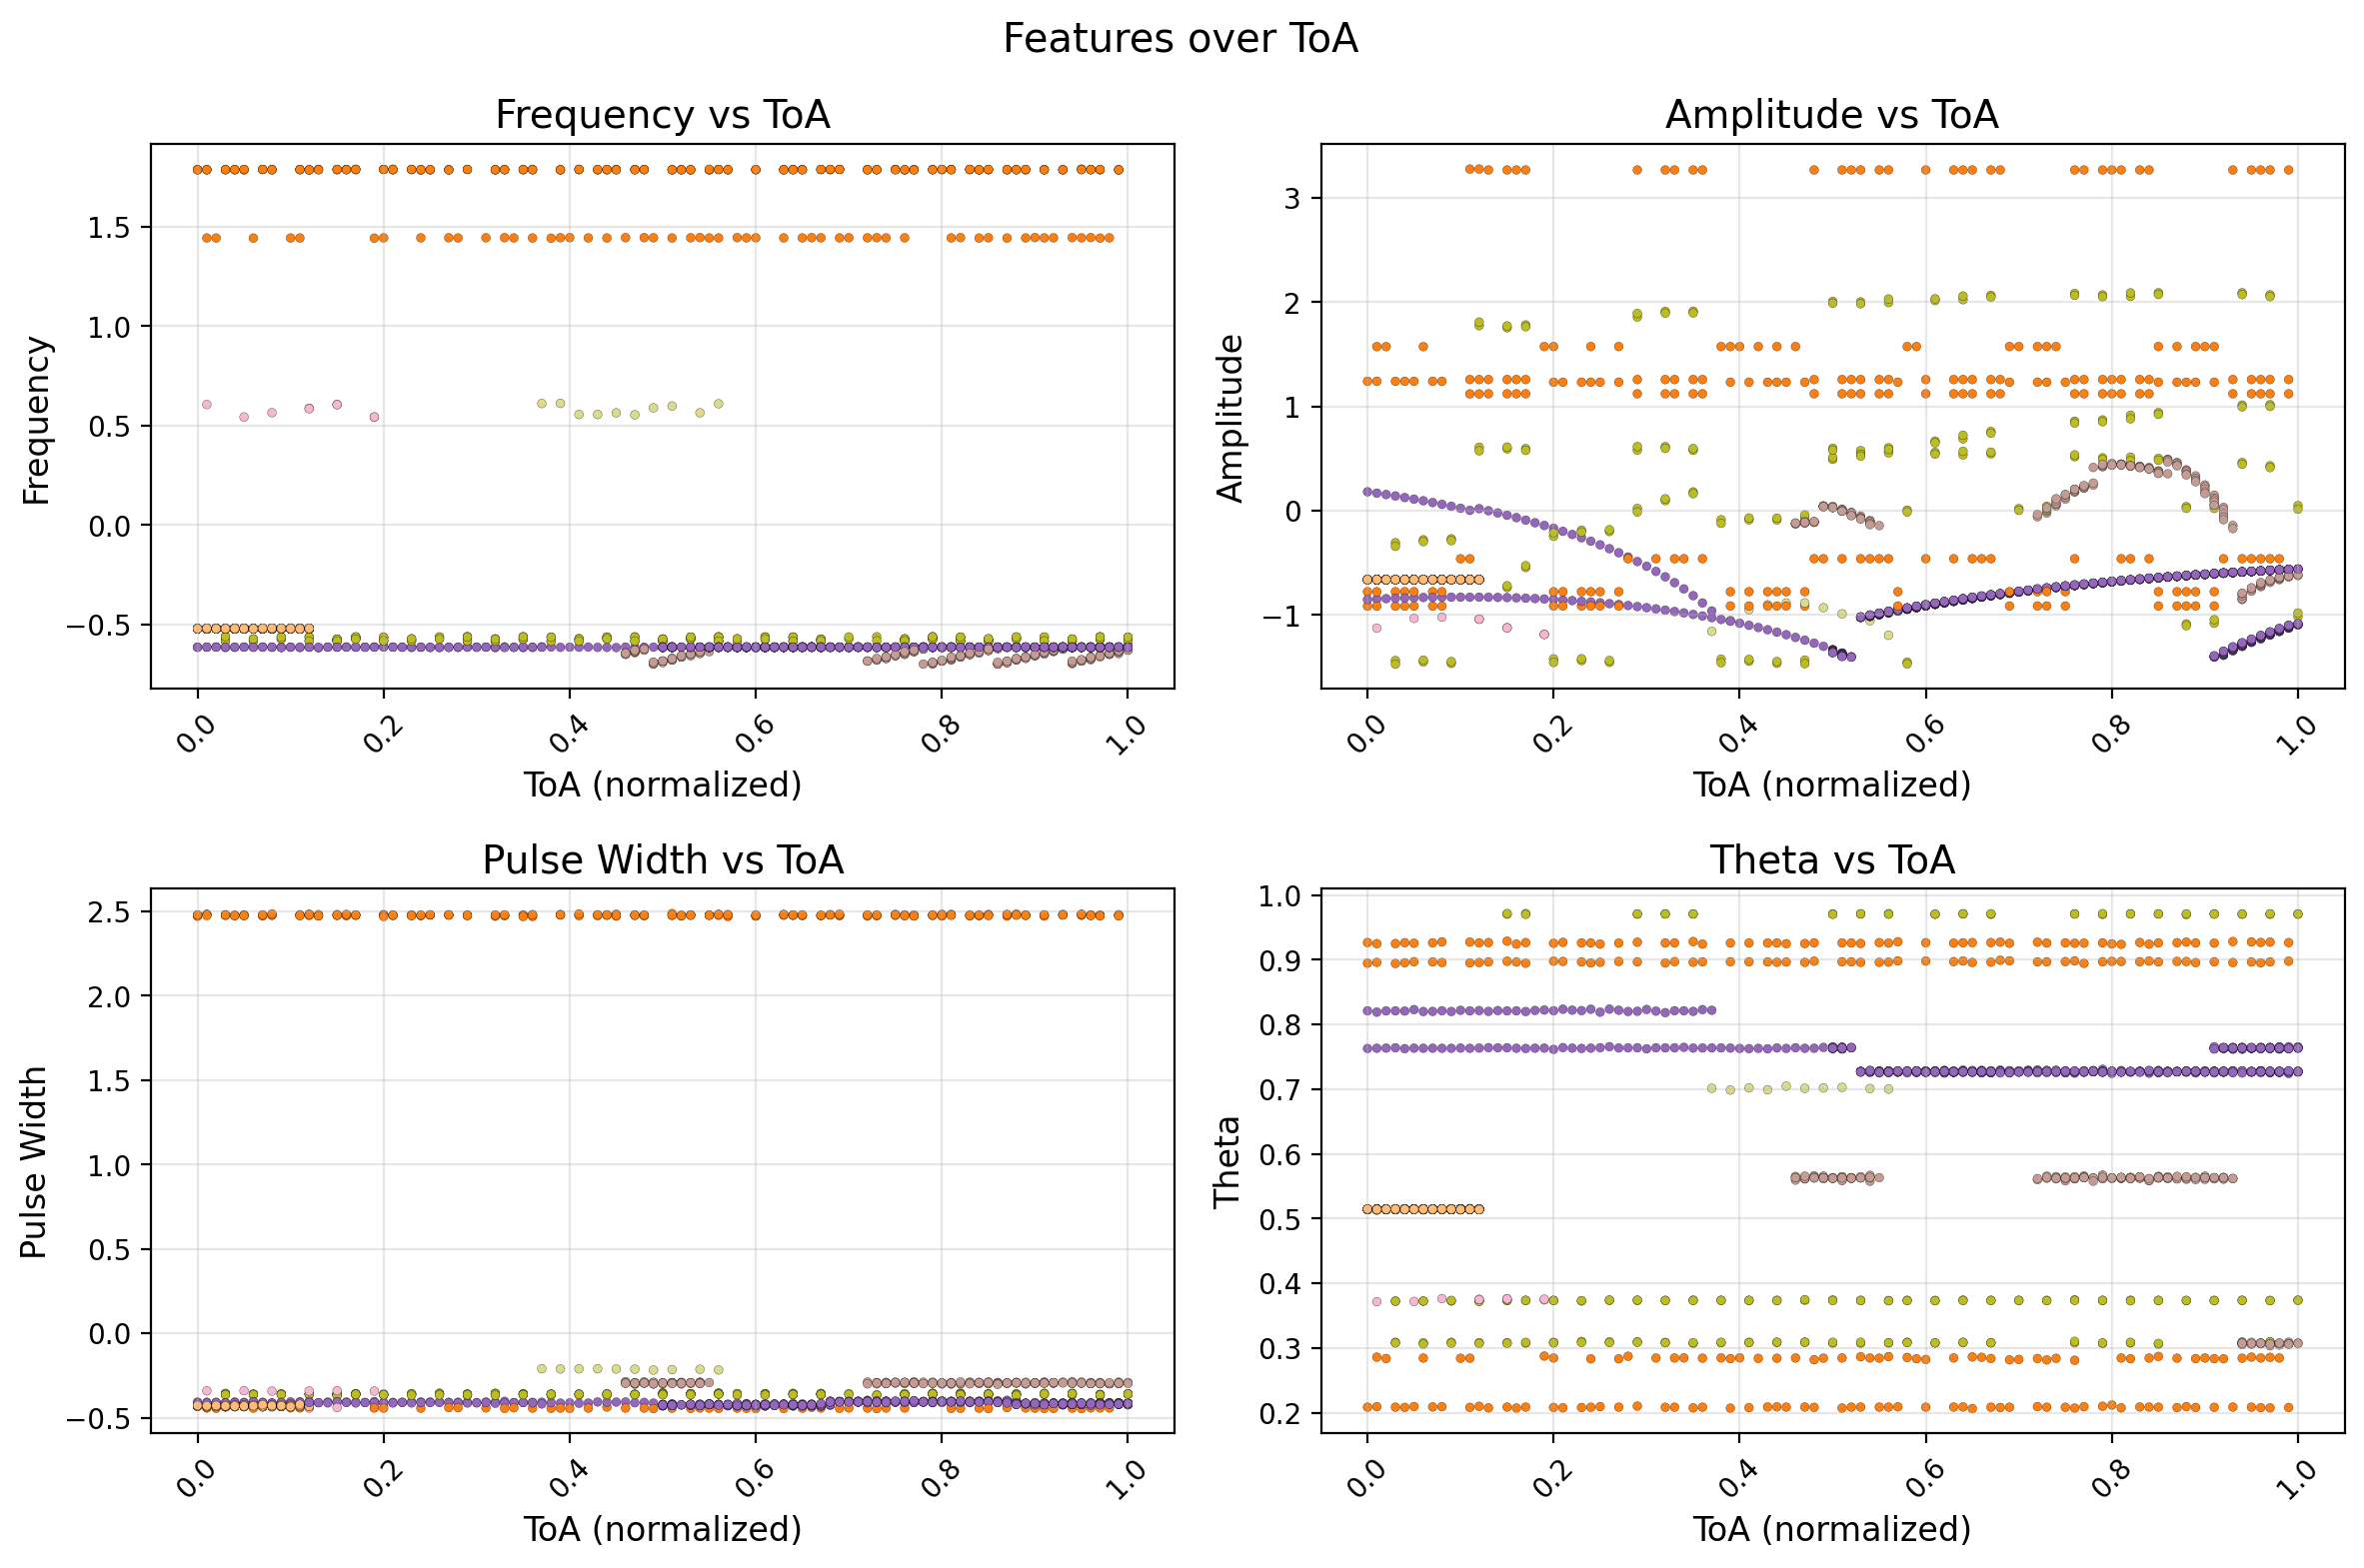
\includegraphics[width=\linewidth,height=0.74\textheight,keepaspectratio]{experiments/feat_maxemitters.png}
    \end{column}
    \begin{column}{0.33\textwidth}
      \centering
      {\small\bfseries Imbalance}\\[0.25em]
      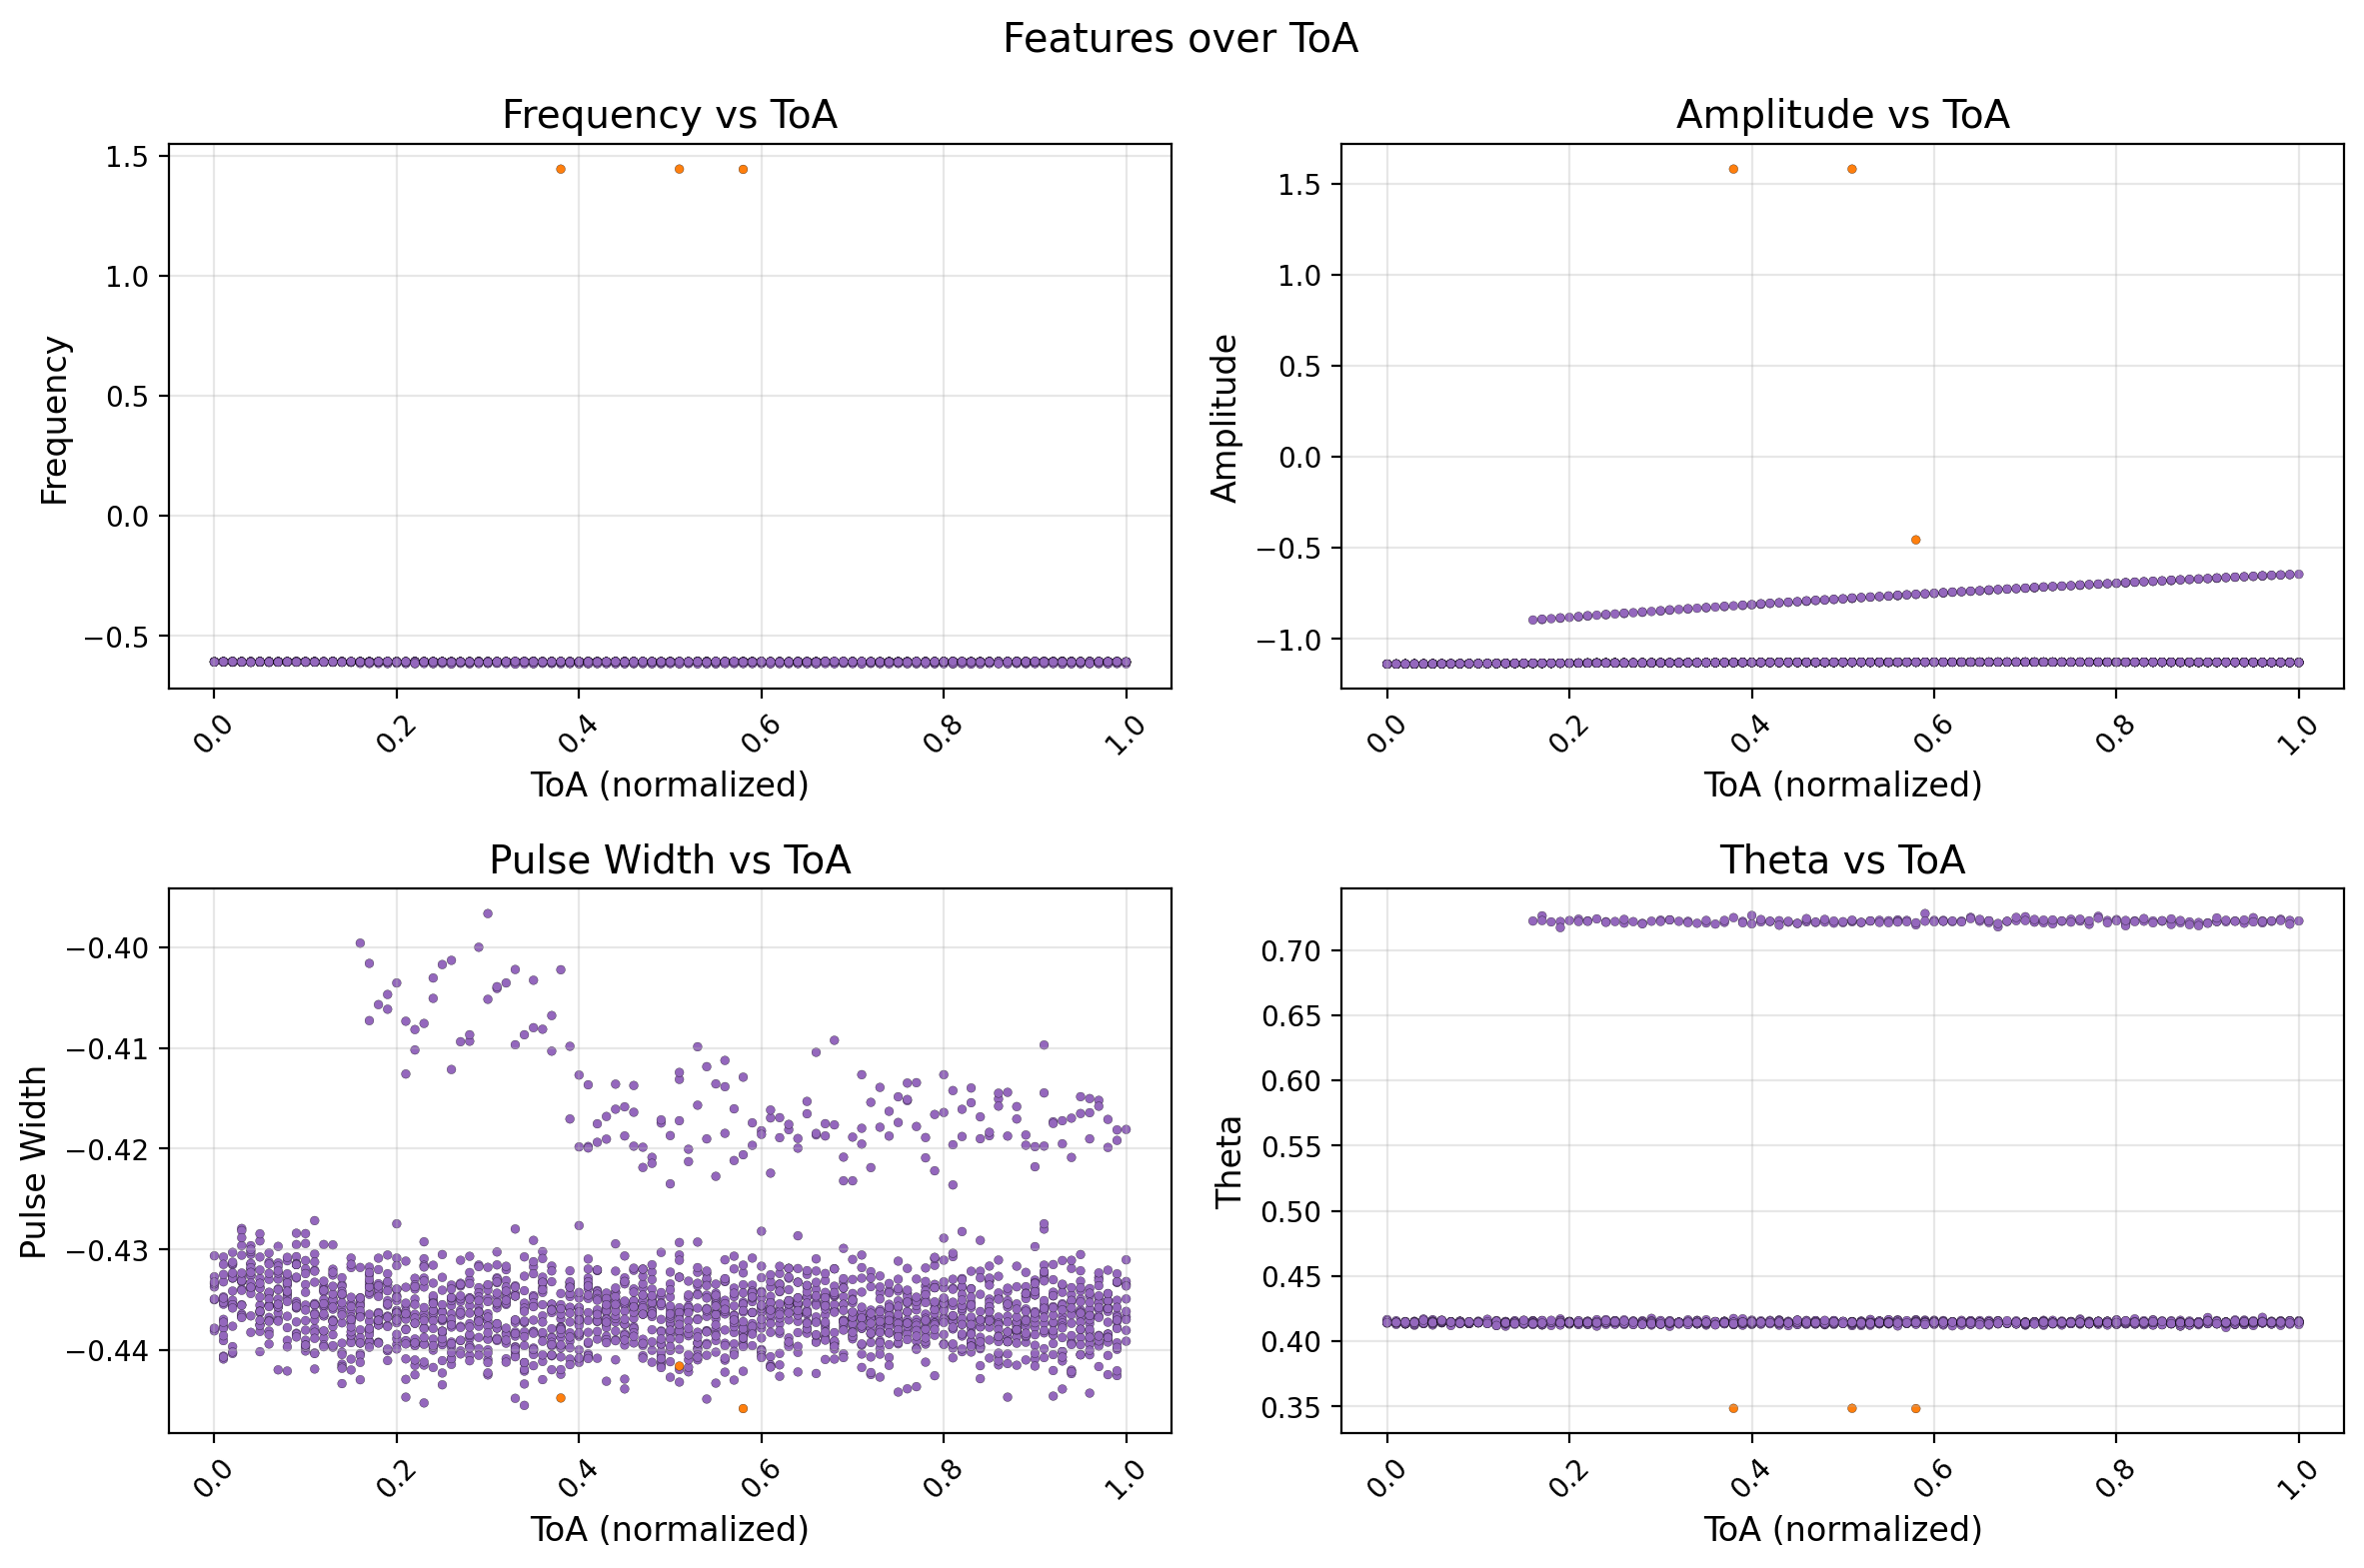
\includegraphics[width=\linewidth,height=0.74\textheight,keepaspectratio]{experiments/feat_imbalance.png}
    \end{column}
    \begin{column}{0.33\textwidth}
      \centering
      {\small\bfseries Sparse}\\[0.25em]
      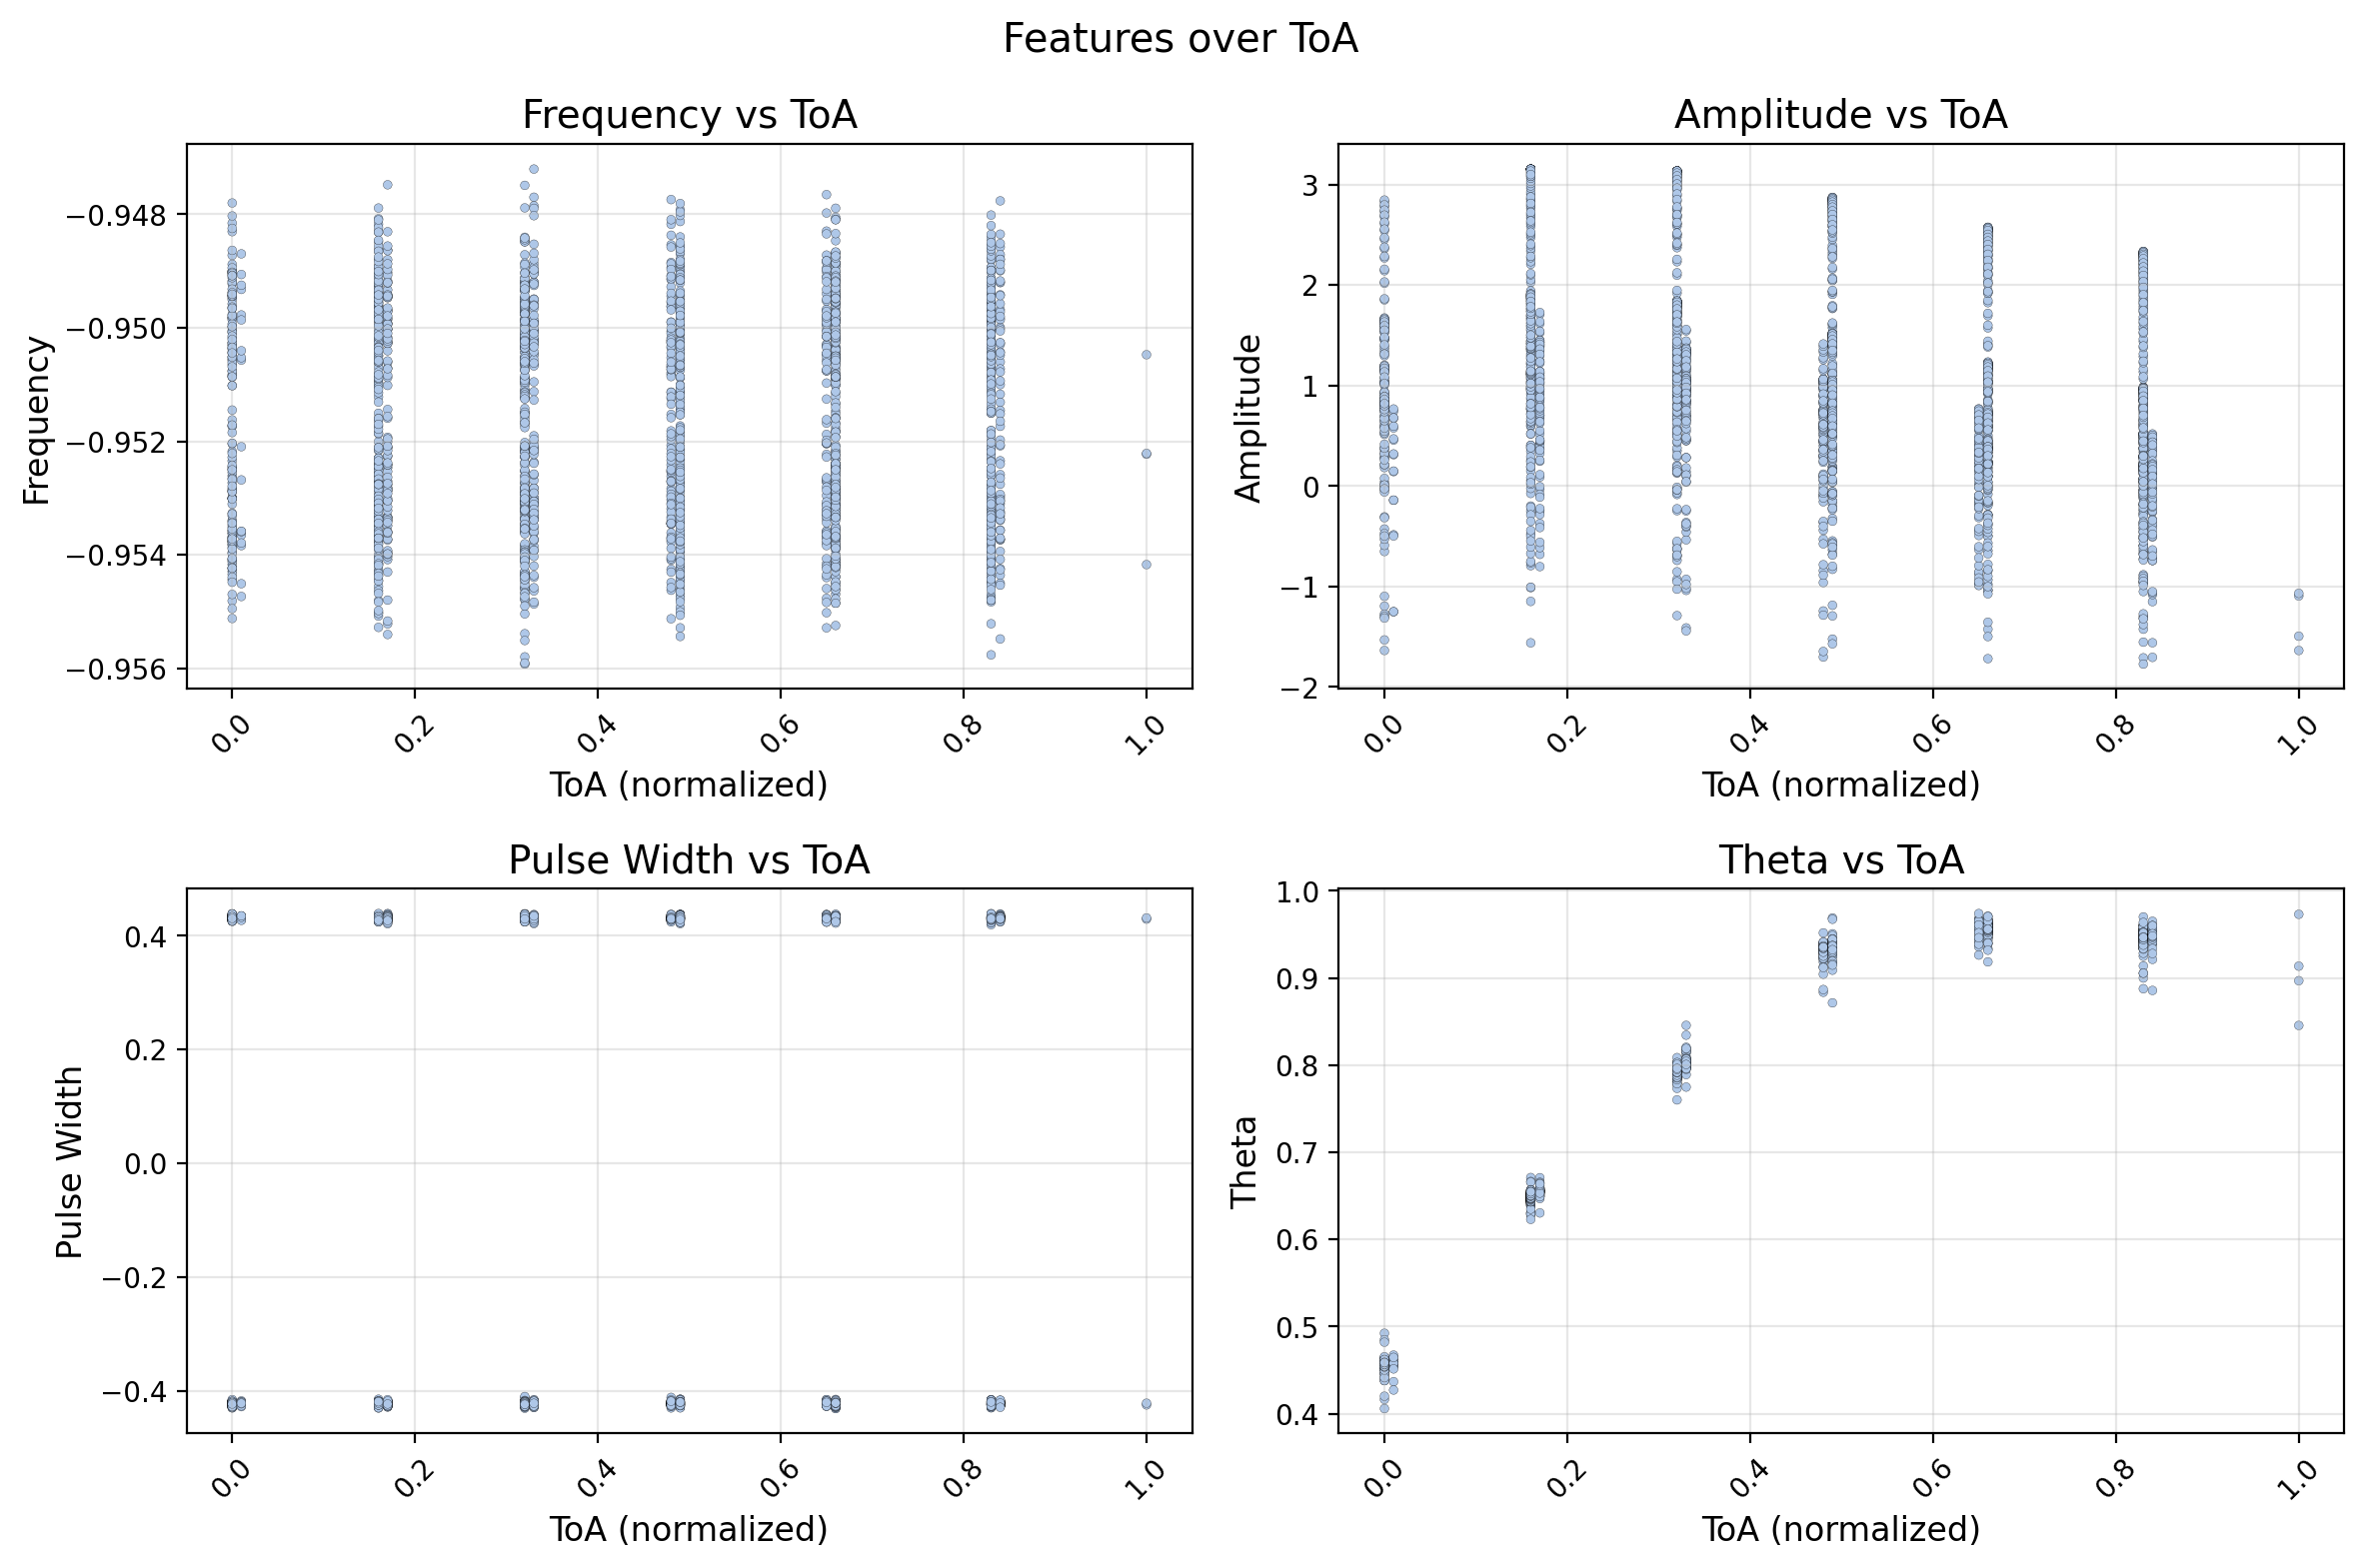
\includegraphics[width=\linewidth,height=0.74\textheight,keepaspectratio]{experiments/feat_scan.png}
    \end{column}
  \end{columns}
  \note{Walk the amplitude panel of the sparse window. Gaps between the lobes are the scan.}
\end{frame}

% ---------------------------------------------------------------------
\begin{frame}{Model architecture}
  \begin{columns}[T,onlytextwidth]
    \begin{column}{0.60\textwidth}
      \textbf{Transformer encoder}
      \begin{itemize}
        \item Input: \(L\) (sequence length) \(\times\) \(F\) (feature dimension)
        \item Output embeddings: \(L \times D\), with \(D = 256\)
      \end{itemize}
      \vspace{0.3em}
      \begin{columns}[T]
        \begin{column}{0.48\textwidth}
          \begin{block}{Strengths}
            \begin{itemize}
              \item A strong sequence model
              \item Returns an embedding per pulse
              \item Widely studied
            \end{itemize}
          \end{block}
        \end{column}
        \begin{column}{0.48\textwidth}
          \begin{alertblock}{Weaknesses}
            \begin{itemize}
              \item \(O(L^{2})\) memory and compute
              \item Long streams must be windowed
              \item Order is not built in
            \end{itemize}
          \end{alertblock}
        \end{column}
      \end{columns}
    \end{column}
    \begin{column}{0.38\textwidth}
      \centering
      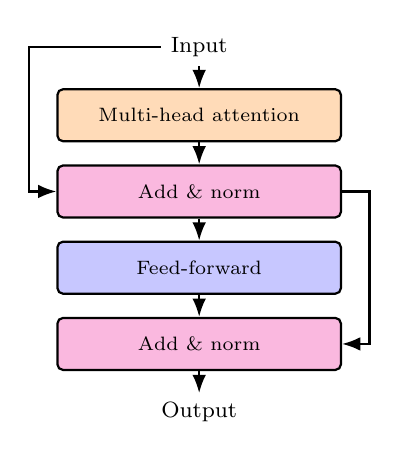
\begin{tikzpicture}[
          font=\scriptsize,
          >=Latex,
          node distance=2.8mm,
          box/.style={draw, thick, rounded corners=2pt, align=center,
                      minimum width=36mm, minimum height=6.6mm, inner sep=2pt},
          arr/.style={->, thick},
        ]
        \node[font=\footnotesize] (inp) {Input};
        \node[box, fill=orange!28, below=of inp] (mha) {Multi-head attention};
        \node[box, fill=magenta!28, below=of mha] (an1) {Add \& norm};
        \node[box, fill=blue!22, below=of an1] (ff) {Feed-forward};
        \node[box, fill=magenta!28, below=of ff] (an2) {Add \& norm};
        \node[font=\footnotesize, below=of an2] (out) {Output};
        \draw[arr] (inp) -- (mha);
        \draw[arr] (mha) -- (an1);
        \draw[arr] (an1) -- (ff);
        \draw[arr] (ff) -- (an2);
        \draw[arr] (an2) -- (out);
        \draw[arr] (inp.west) -- ([xshift=-3.5mm]mha.west |- inp.west)
          -- ([xshift=-3.5mm]mha.west |- an1.west) -- (an1.west);
        \draw[arr] (an1.east) -- ([xshift=3.5mm]mha.east |- an1.east)
          -- ([xshift=3.5mm]mha.east |- an2.east) -- (an2.east);
      \end{tikzpicture}
    \end{column}
  \end{columns}
\end{frame}

% ---------------------------------------------------------------------
\begin{frame}{Shared trunk, two heads, two positive sets}
  \begin{columns}[c,onlytextwidth]
    \begin{column}{0.46\textwidth}
      \centering
      \thesisfig{!}{0.86\textheight}{../figures/method/architecture.tex}
    \end{column}
    \begin{column}{0.52\textwidth}
      \begin{itemize}
        \item The trunk and both branches are stacks of transformer encoder layers.
        \item A projection head reduces the dimension before \(\ell_2\) normalization.
        \item 16.1 million parameters.
        \item DBSCAN is applied to the embeddings at inference.
        \item Training does not run DBSCAN. The loss uses the embeddings directly.
      \end{itemize}
    \end{column}
  \end{columns}
  \note{The two similarities can fight in the trunk.}
\end{frame}

% ---------------------------------------------------------------------
\begin{frame}{Attention mechanism}
  \begin{columns}[c,onlytextwidth]
    \begin{column}{0.40\textwidth}
      \centering
      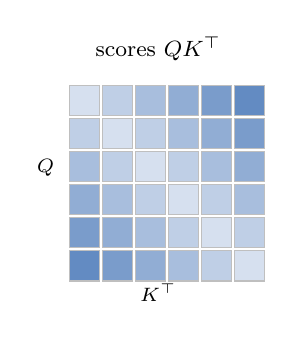
\begin{tikzpicture}[x=0.42cm,y=0.42cm,font=\scriptsize]
        \foreach \i in {0,...,5} {
          \foreach \j in {0,...,5} {
            \pgfmathsetmacro{\tone}{18+10*abs(\i-\j)}
            \fill[kthblue!\tone] (\j,-\i) rectangle ++(0.92,-0.92);
            \draw[black!25] (\j,-\i) rectangle ++(0.92,-0.92);
          }
        }
        \node[anchor=south, font=\footnotesize] at (2.7,0.45) {scores \(QK^{\top}\)};
        \node[anchor=east] at (-0.15,-2.5) {\(Q\)};
        \node[anchor=north] at (2.7,-5.7) {\(K^{\top}\)};
      \end{tikzpicture}

      \vspace{0.6em}
      {\footnotesize A similarity matrix: a complete weighted graph on the \(L\) pulses.}
    \end{column}
    \begin{column}{0.58\textwidth}
      \[
        \mathrm{Attention}(Q,K,V)
        = \softmax\!\left(\frac{QK^{\top}}{\sqrt{d}}\right) V
      \]
      \begin{itemize}
        \item Each row of \(QK^{\top}\) scores one pulse against every other pulse in the window.
        \item Softmax turns that row into weights. The pulse is then a mixture of the values \(V\).
        \item Nothing in this product knows the order of the pulses, or their TOA.
      \end{itemize}
    \end{column}
  \end{columns}
\end{frame}

% ---------------------------------------------------------------------
\begin{frame}{Two ways to put position into attention}
  \begin{columns}[T,onlytextwidth]
    \begin{column}{0.49\textwidth}
      \begin{block}{Rotary encodings (RoPE-TOA)}
        \begin{itemize}
          \item Rotate \(Q\) and \(K\) by the window-local TOA.
          \item The score is a dot product, so only the enclosed angle matters.
          \item Only the relative rotation \(R(\Delta t)\) enters the product.
          \item In language models the angle is the token index. Here it is TOA, because PDWs are not equally spaced.
          \item No extra memory, and about \(O(L)\) extra compute.
        \end{itemize}
      \end{block}
    \end{column}
    \begin{column}{0.49\textwidth}
      \begin{alertblock}{Physical bias}
        \begin{itemize}
          \item Build \(B_{ij} = \lvert p_i - p_j \rvert\) from TOA and incidence.
          \item Scale by a learned \(\lambda\) and subtract from the attention logits.
          \item One \(\lambda\) per head and per stack, so heads can penalize or reward different deltas.
          \item \(O(L^{2})\) compute and memory, the same order as attention itself.
          \item Uncommon in language models, because of that quadratic cost.
        \end{itemize}
      \end{alertblock}
    \end{column}
  \end{columns}
\end{frame}

% ---------------------------------------------------------------------
\begin{frame}{RoPE-TOA: each plane rotates at its own frequency}
  \centering
  \thesisfig{0.78\textwidth}{!}{../figures/background/rope_rotation.tex}

  \vspace{0.15em}
  \begin{columns}[T,onlytextwidth]
    \begin{column}{0.32\textwidth}
      \centering
      {\small One head is split into 2D planes. Each plane has its own frequency.}
    \end{column}
    \begin{column}{0.32\textwidth}
      \centering
      {\small Equal TOA leaves \(Q\) and \(K\) as they are. It does not pull them together or apart.}
    \end{column}
    \begin{column}{0.32\textwidth}
      \centering
      {\small The score keeps only the relative gap, which twists the fast planes more.}
    \end{column}
  \end{columns}
  \note{Four 2D planes of one head; the left plane is the fastest. A shared TOA cancels, so the angle between Q and K is unchanged. Only the relative time gap rotates one against the other, and it twists the fast planes more.}
\end{frame}

% ---------------------------------------------------------------------
\begin{frame}{Physical bias: learned \(\lambda\) on delta maps}
  \begin{columns}[c,onlytextwidth]
    \begin{column}{0.64\textwidth}
      \centering
      {\scriptsize
      \begin{tabular}{@{}c@{\;\;}c@{\;\;}c@{\;\;}c@{\;\;}c@{}}
        \deltagrid{teal} &
        \(+\) &
        \groupgrid{orange} &
        \(=\) &
        \deltagrid{violet} \\[0.35em]
        \(\lvert\Delta\mathrm{TOA}\rvert\cdot\lambda_t\) & &
        \(\lvert\Delta\mathrm{incidence}\rvert\cdot\lambda_u\) & &
        bias \(\lambda B\) \\[0.9em]
        \deltagrid{kthblue} &
        \(-\) &
        \deltagrid{violet} &
        \(=\) &
        
\begin{tikzpicture}[x=0.42cm,y=0.42cm,baseline=-0.5ex]
          \foreach \i in {0,...,4} {%
            \foreach \j in {0,...,4} {%
              \pgfmathtruncatemacro{\keep}{max(12,80-16*abs(\i-\j))}%
              \fill[kthblue!\keep] (\j,-\i) rectangle ++(0.92,-0.92);%
            }%
          }%
        \end{tikzpicture} \\[0.35em]
        attention \(A\) & &
        \(\lambda B\) & &
        \(A - \lambda B\)
      \end{tabular}}

      \vspace{0.45em}
      {\footnotesize Nearby, same-direction pulses stay bright. The maps are \(L \times L\). That is the cost.}
    \end{column}
    \begin{column}{0.34\textwidth}
      \begin{itemize}
        \item \(\lvert\Delta\mathrm{TOA}\rvert\) and \(\lvert\Delta\mathrm{incidence}\rvert\) come from the inputs.
        \item \(\lambda_t\) and \(\lambda_u\) are learned scalars, one pair per head.
        \item The bias is subtracted from the vanilla logits.
        \item A cache can skip rebuilding \(B\). It does not skip the quadratic subtract.
      \end{itemize}
    \end{column}
  \end{columns}
  \note{A cache skips the rebuild, not the quadratic subtract. RoPE is the cheaper of the two.}
\end{frame}

% ---------------------------------------------------------------------
\begin{frame}{Loss function}
  Supervised contrastive loss. Pulses that share a label are the positives. Every other pulse in the batch is a candidate.

  \vspace{0.15em}
  {\small
  \[
    s_{ij} \coloneqq \vect{z}_i^{\top}\vect{z}_j \in [-1,1]
  \]
  \[
    \Loss_{\mathrm{SC}}
    = -\sum_{i \in \mathcal{B}^{+}} \frac{1}{\lvert P(i)\rvert}
      \sum_{p \in P(i)}
      \log \frac{\exp(s_{ip}/\tau)}{\sum_{a \in A(i)}\exp(s_{ia}/\tau)}
  \]}

  \vspace{0.15em}
  {\footnotesize
  \(A(i)\) is every pulse in the batch except \(i\).
  \(P(i)\subseteq A(i)\) is those that share its label.
  \(\mathcal{B}^{+}\) is the pulses with at least one positive.
  \(\tau = 0.5\).}

  \vspace{0.45em}
  The same expression separates into repulsion and attraction:
  {\small
  \[
    \Loss_{\mathrm{SC}}
    =
    \underbrace{\sum_{i\in\mathcal{B}^{+}}\log Z_i}_{\text{log-partition (repulsion)}}
    -
    \underbrace{\sum_{i\in\mathcal{B}^{+}}\frac{1}{\lvert P(i)\rvert}
      \sum_{p\in P(i)}\frac{s_{ip}}{\tau}}_{\text{mean positive similarity (attraction)}},
    \quad
    Z_i = \sum_{a'\in A(i)}\exp(s_{ia'}/\tau).
  \]}
\end{frame}

% ---------------------------------------------------------------------
\begin{frame}{Joint training}
  \vspace{0.4em}
  \[
    \Loss_{\mathrm{joint}} = \Loss_{\mathrm{em}} + \Loss_{\mathrm{md}}.
  \]
  \vspace{0.2em}
  \begin{itemize}
    \item The two terms are the same loss on different positive sets.
    \item Emitter positives share a recording-local emitter identity, so the term trains deinterleaving.
    \item Mode positives share a catalogue mode, and the comparison runs across the batch.
  \end{itemize}
  \vspace{0.4em}
  Task-specific models keep the same two branches but train on one term only.
  The other branch is still computed and then discarded, which is a pure deinterleaving transformer or a pure mode transformer.
\end{frame}

% ---------------------------------------------------------------------
\begin{frame}{Deinterleaving: mean \(\pm\) std over 1169 windows}
  {\small Joint training. Feature DBSCAN, with no encoder, has ARI \(0.578\pm0.348\) and count error \(7.04\pm5.85\).}
  \vspace{0.45em}
  \centering
  {\small
  \begin{tabular}{@{}lcc@{}}
    \toprule
    Model & ARI & Count error \\
    \midrule
    Vanilla       & \(0.948\pm0.176\) & \(0.25\pm0.49\) \\
    RoPE-TOA      & \(\mathbf{1.000\pm0.003}\) & \(0.11\pm0.34\) \\
    RoPE-az       & \(0.973\pm0.135\) & \(0.16\pm0.40\) \\
    Bias          & \(\mathbf{1.000\pm0.002}\) & \(\mathbf{0.10\pm0.33}\) \\
    RoPE-TOA+Bias & \(0.851\pm0.255\) & \(0.73\pm0.94\) \\
    \bottomrule
  \end{tabular}}

  \vspace{0.8em}
  {\small Joint versus emitter-only.}
  \vspace{0.35em}
  \centering
  {\small
  \begin{tabular}{@{}lcc@{}}
    \toprule
    Model & Joint ARI & Emitter-only ARI \\
    \midrule
    Vanilla  & \(0.948\pm0.176\) & \(0.999\pm0.012\) \\
    RoPE-TOA & \(1.000\pm0.003\) & \(0.998\pm0.036\) \\
    Bias     & \(1.000\pm0.002\) & \(0.840\pm0.265\) \\
    \bottomrule
  \end{tabular}}
\end{frame}

\begin{frame}{Mode clustering: mean \(\pm\) std over 1169 windows}
  {\small Joint training. Feature DBSCAN has ARI \(0.811\pm0.250\) and count error \(4.99\pm3.99\).}
  \vspace{0.45em}
  \centering
  {\small
  \begin{tabular}{@{}lcc@{}}
    \toprule
    Model & ARI & Count error \\
    \midrule
    Vanilla       & \(0.985\pm0.107\) & \(0.23\pm0.50\) \\
    RoPE-TOA      & \(0.991\pm0.075\) & \(0.20\pm0.48\) \\
    RoPE-az       & \(0.983\pm0.102\) & \(0.24\pm0.51\) \\
    Bias          & \(\mathbf{0.992\pm0.081}\) & \(\mathbf{0.14\pm0.41}\) \\
    RoPE-TOA+Bias & \(0.977\pm0.112\) & \(0.32\pm0.60\) \\
    \bottomrule
  \end{tabular}}

  \vspace{0.8em}
  {\small Joint versus mode-only on the Vanilla encoder.}
  \vspace{0.35em}
  \centering
  {\small
  \begin{tabular}{@{}lcc@{}}
    \toprule
    Objective & ARI & Count error \\
    \midrule
    Joint     & \(\mathbf{0.985\pm0.107}\) & \(\mathbf{0.23\pm0.50}\) \\
    Mode-only & \(0.983\pm0.110\) & \(0.24\pm0.56\) \\
    \bottomrule
  \end{tabular}}
\end{frame}

% ---------------------------------------------------------------------
\begin{frame}{Distribution of scores over windows}
  {\small Logarithmic vertical axis. A curve that stays low until 1 is better. Dashed: single-task.}

  \vspace{0.15em}
  \begin{columns}[c,onlytextwidth]
    \begin{column}{0.50\textwidth}
      \centering
      {\small\bfseries Deinterleaving}\\[0.15em]
      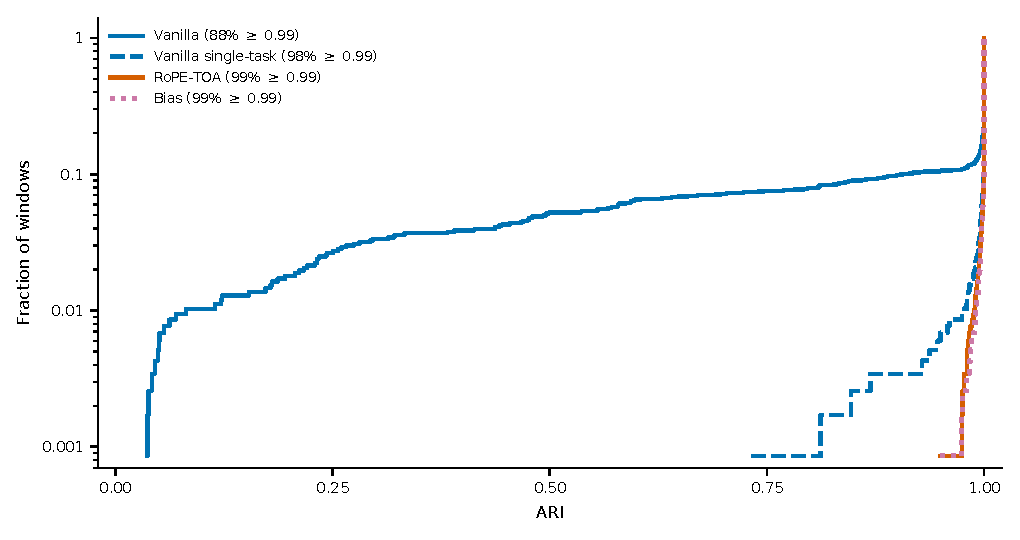
\includegraphics[width=\linewidth,height=0.74\textheight,keepaspectratio]{experiments/hist_em_all.pdf}
    \end{column}
    \begin{column}{0.50\textwidth}
      \centering
      {\small\bfseries Mode clustering}\\[0.15em]
      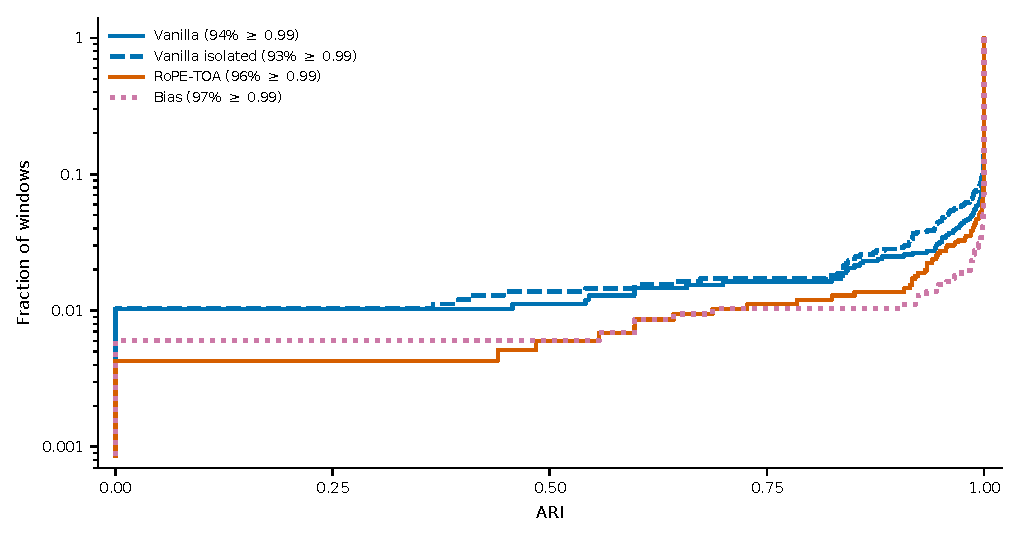
\includegraphics[width=\linewidth,height=0.74\textheight,keepaspectratio]{experiments/hist_md_all.pdf}
    \end{column}
  \end{columns}
  \note{The deinterleaving question is yes, with a leftover tail on the joint vanilla model. Mode is already easier in the raw PDWs.}
\end{frame}

% ---------------------------------------------------------------------
\begin{frame}{Conclusion}
  \begin{block}{Deinterleaving}
    \begin{itemize}
      \item The joint model is weaker than the single-task model when attention is left unmodified.
      \item With RoPE-TOA or the physical bias, the joint model is on par with single-task deinterleaving, and slightly ahead.
    \end{itemize}
  \end{block}
  \vspace{0.6em}
  \begin{block}{Mode clustering}
    The joint model is slightly better than the single-task model, and the two are essentially on par.
  \end{block}
\end{frame}

% ---------------------------------------------------------------------
\begin{frame}{Discussion and further work}
  \begin{columns}[T,onlytextwidth]
    \begin{column}{0.50\textwidth}
      \textbf{Windows}
      \begin{itemize}
        \item A scenario is longer than one window.
        \item The window clusters still have to be stitched into a scenario-level answer.
      \end{itemize}
      \vspace{0.8em}
      \textbf{A second head}
      \begin{itemize}
        \item A mode classification head could sit on the mode embeddings, beside the clustering path.
      \end{itemize}
    \end{column}
    \begin{column}{0.48\textwidth}
      \centering
      \thesisfig{!}{0.70\textheight}{../figures/method/architecture.tex}\\[0.2em]
      {\footnotesize A classification head would read the mode embeddings \(\vect{z}^{\mathrm{md}}_n\).}
    \end{column}
  \end{columns}
\end{frame}

% ---------------------------------------------------------------------
\begin{frame}
  \vfill
  \centering
  {\usebeamercolor[fg]{title}\Huge\bfseries Questions?\par}
  \vfill
\end{frame}

\end{document}
